\documentclass[11pt,a4paper]{article}
\usepackage{amsmath,amsthm,amsfonts,amssymb,amscd}
\usepackage{enumerate} 
\usepackage{physics}
\usepackage{enumerate}
\usepackage{fancyhdr}
 \usepackage{hyperref}
\hypersetup{colorlinks,
    linkcolor=blue,
    citecolor=blue,      
    urlcolor=blue,
}
\usepackage{graphicx}


\oddsidemargin0.1cm 
\evensidemargin0.8cm
\textheight22.7cm 
\textwidth15cm \topmargin-0.5cm

\newtheorem{theorem}{Theorem}[section]
\newtheorem{lemma}[theorem]{Lemma}

\usepackage{listings}
\usepackage{xcolor}

\definecolor{codegreen}{rgb}{0,0.6,0}
\definecolor{codegray}{rgb}{0.5,0.5,0.5}
\definecolor{codepurple}{rgb}{0.58,0,0.82}
\definecolor{backcolour}{rgb}{0.95,0.95,0.92}

\lstdefinestyle{mystyle}{
    backgroundcolor=\color{backcolour},   
    commentstyle=\color{codegreen},
    keywordstyle=\color{magenta},
    numberstyle=\tiny\color{codegray},
    stringstyle=\color{codepurple},
    basicstyle=\ttfamily\footnotesize,
    breakatwhitespace=false,         
    breaklines=true,                 
    captionpos=b,                    
    keepspaces=true,                 
    numbers=left,                    
    numbersep=5pt,                  
    showspaces=false,                
    showstringspaces=false,
    showtabs=false,                  
    tabsize=2
}

\lstset{style=mystyle}

\newcommand{\silvia}[1]{{ {\color{blue}{(silvia)~#1}}}}
\newcommand{\grace}[1]{{ {\color{purple}{(grace)~#1}}}}

\newcommand{\MultiSet}{\mathrm{MultiSet}}
\newcommand{\len}{\mathrm{len}}
\newcommand{\din}{\texttt{d\_in}}
\newcommand{\dout}{\texttt{d\_out}}
\newcommand{\T}{\texttt{T} }
\newcommand{\F}{\texttt{F} }
\newcommand{\Relation}{\texttt{Relation}}
\newcommand{\X}{\mathcal{X}}
\newcommand{\Y}{\mathcal{Y}}
\newcommand{\True}{\texttt{True}}
\newcommand{\False}{\texttt{False}}
\newcommand{\clamp}{\texttt{clamp}}
\newcommand{\function}{\texttt{function}}
\newcommand{\float}{\texttt{float }}
\newcommand{\questionc}[1]{\textcolor{red}{\textbf{Question:} #1}}

\title{Privacy Proofs for OpenDP: Impute Uniform Float Transformation}
\author{Grace Tian}
\date{Summer 2021}
\begin{document}

\maketitle
\tableofcontents

\section{Algorithm Implementation}
\subsection{Code in Rust}

The current OpenDP library contains the \texttt{make\_impute\_uniform\_float} function implementing the impute uniform float function. This is defined in lines 14-30 of the file \texttt{impute.rs} in the Git repository \url{https://github.com/opendp/opendp/blob/21-impute/rust/opendp/src/trans/impute.rs#L14-L30}



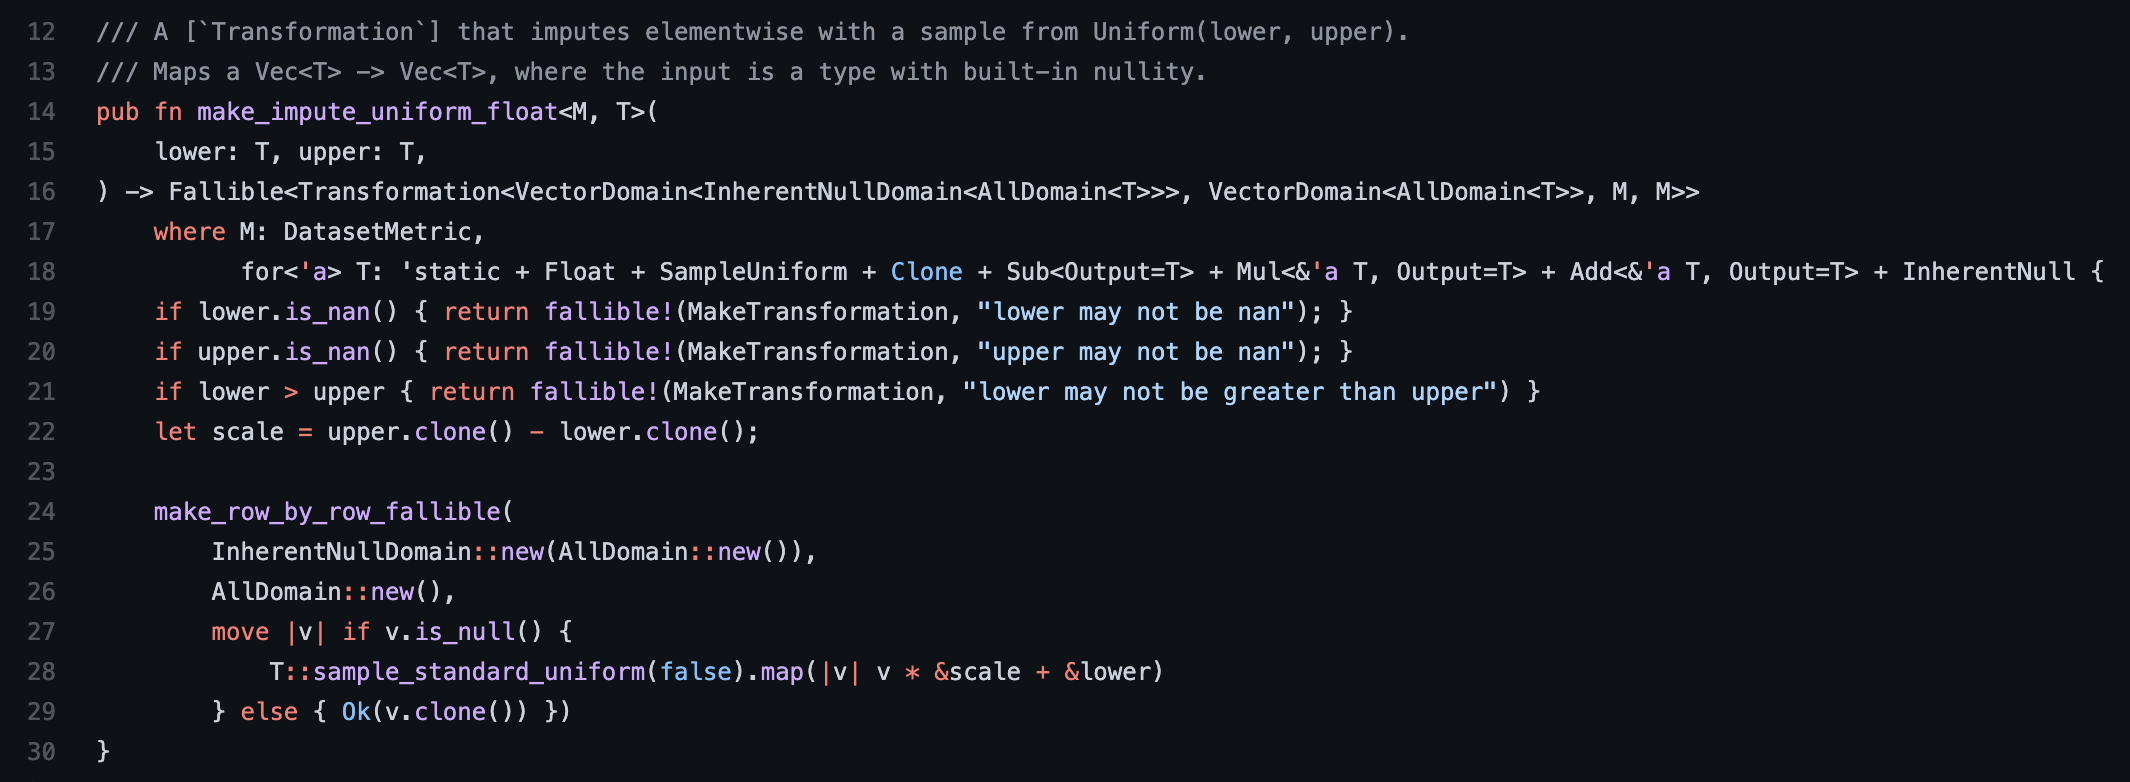
\includegraphics[width=\textwidth]{make_impute_unif_float.png}


\subsection{Pseudo Code in Python}

\subsubsection*{Preconditions}
To ensure the correctness of the output, we require the following preconditions:

\begin{itemize}
    \item \textbf{User-specified types:}
    \begin{itemize}
        \item Variables \texttt{lower} and \texttt{upper} must be of type \T
        \item Type \texttt{T} must have traits \texttt{float}, \texttt{SampleUniform}, \texttt{Clone}, \texttt{Sub(Output=T)}, \texttt{Mul}, \texttt{Add}, and \texttt{InherentNull}.
    \end{itemize}
\end{itemize}

\subsubsection*{Postconditions}
\begin{itemize}
    \item A \texttt{Transformation} is returned (i.e., if a \texttt{Transformation} cannot be returned successfully, then an error should be returned).
\end{itemize}


\begin{lstlisting}[language=Python, escapechar=|]
def make_impute_uniform_float(lower : T, upper : T):
    input_domain = VectorDomain(InherentNullDomain(AllDomain(T)));
    output_domain = VectorDomain(AllDomain(T))
    input_metric = SymmetricDistance()
    output_metric = SymmetricDistance()

    def Relation(d_in: u32, d_out: u32) -> bool: |\label{line:rel}|
        return d_out >= d_in*1
    
    # should input to function include inherent null?
    def function(data : Vec(T)) -> Vec(T): 
        return list(map(Uniform(lower, upper), data))

    let stability_relation = (d_in <= d_out);
    
    return Transformation(input_domain, output_domain, function, input_metric, output_metric, stability_relation)
    # TODO replace with return row_by_row_fallible

\end{lstlisting}




\section{Proof}
\begin{theorem}


For every setting of the input parameters \texttt{(lower, upper)} to \texttt{make\_impute\_uniform\_float} such that the given preconditions hold, the transformation returned by \texttt{make\_impute\_uniform\_float} has the following properties:
\begin{enumerate}
    \item \textup{(Appropriate output domain).} If vector $v$ is in the \texttt{input\_domain}, then \texttt{function(v)} is in the \texttt{output\_domain}.
    \item \textup{(Domain-Metric Compatibility).} The domain \texttt{input\_domain} matches one of the possible domains listed in the definition of \texttt{input\_metric}, and likewise \texttt{output\_domain} matches one of the possible domains listed in the definition of \texttt{output\_metric}.
    \item \textup{(Stability Guarantee).} For every pair of elements $v, w$ in \texttt{input\_domain} and for every pair $(\din, \dout)$, where $\din$ is of the associated type for \texttt{input\_metric} and $\dout$ is the associated type for \texttt{output\_metric}, if $v,w$ are $d_{in}$-close under \texttt{input\_metric} and $\Relation(\din, \dout) = \True$, then $\function(v), \function(w)$ are $d_{out}$-close under \texttt{output\_metric}.
\end{enumerate}
\end{theorem}

\begin{proof}
\begin{enumerate}
    \item \textbf{(Appropriate output domain).} In the case of \texttt{make\_impute\_uniform\_float}, this corresponds to showing that for every vector $v$ of elements of type \texttt{InherentNullDomain(T)} \grace{T? or InherentNullDomain???}, \texttt{function}$(v)$ is a vector of elements of type \texttt{T}. 
    
    \grace{TODO We show the type signature + nullity works}
    
    \item \textbf{(Domain-metric compatibility).} The Symmetric distance is both the \texttt{input\_metric} and \texttt{output\_metric}. Symmetric distance is compatible with \texttt{VectorDomain(T)} for any generic type \texttt{T}, as stated in \href{https://www.overleaf.com/project/60d215bf90b337ac02200a99}{``List of definitions used in the pseudocode"}. The theorem holds because for \texttt{make\_impute\_constant}, the input domain is \\ \texttt{VectorDomain(InherentNullDomain(AllDomain(T)))} and the output domain is \texttt{VectorDomain(AllDomain(T))}. 
    \item \textbf{(Stability guarantee).}
    
    We know that vectors $v, w$ are $d_{in}$-close, and that $d_{in} \leq d_{out}$ because \texttt{Relation}($d_{in}$, $d_{out}$) \texttt{= True}. By the histogram notation, this means that $$d_{Sym}(v, w) = \norm{h_v - h_w}_1 = \sum_{z} \abs{h_v(z) - h_w(z)} \leq d_{in}.$$ Recall that the \texttt{make\_impute\_uniform\_float} transformation only changes the null values in the vectors $v$ and $w$. Therefore it suffices to consider only the subset of null elements in $Multiset(v)$ and $Multiset(w)$, which we denote respectively as $v^*$ and $w^*$. 
    
    From the histogram notation, we have $h_v(\texttt{null})$ and $h_w(\texttt{null})$ nulls respectively in vectors $v$ and $w$. By the stability for randomness corollary, we can fix the random seed $r$, and say it produces the sequence $(r_1, r_2, r_3, \ldots)$ of randomly generated uniforms from \texttt{Unif(lower, upper)} in this specific order. In other words, the $i$th \texttt{null} in $v$ or $w$ corresponds to $r_i$ in function(v) or function(w). Therefore the symmetric distance of $\textttt{function}(v^*)$ and  $\texttt{function}(w^*)$ is bounded:
    
    
    $$\sum_{r_i \in r} \abs{h_{\texttt{function}(v^*)}(r_i) - h_{\texttt{function}(w^*)}(r_i)} \leq \abs{h_{v}(\texttt{null}) - h_{w}(\texttt{null})}$$
    
    The remaining non-null values in $v$ and $z$ stay the same after the transformation, so the transformations are $d_{out}$-close: $$d_{sym}(\texttt{function}(v), \texttt{function}(w)) = \sum_z \abs{h_{\texttt{function}(v)}(z) - h_{\texttt{function}(w)}(z)}$$
    $$\leq \sum_z \abs{h_v(z) - h_w(z)} \leq d_{in} \leq d_{out}$$ 
    
    


    
\end{enumerate}
\end{proof}

\end{document}
